% This file was created by matlab2tikz.
%
%The latest updates can be retrieved from
%  http://www.mathworks.com/matlabcentral/fileexchange/22022-matlab2tikz-matlab2tikz
%where you can also make suggestions and rate matlab2tikz.
%
\definecolor{mycolor1}{rgb}{0.00000,0.44700,0.74100}%
\definecolor{mycolor2}{rgb}{0.85000,0.32500,0.09800}%
\definecolor{mycolor3}{rgb}{0.92900,0.69400,0.12500}%
\definecolor{mycolor4}{rgb}{0.49400,0.18400,0.55600}%
\definecolor{mycolor5}{rgb}{0.46600,0.67400,0.18800}%
%
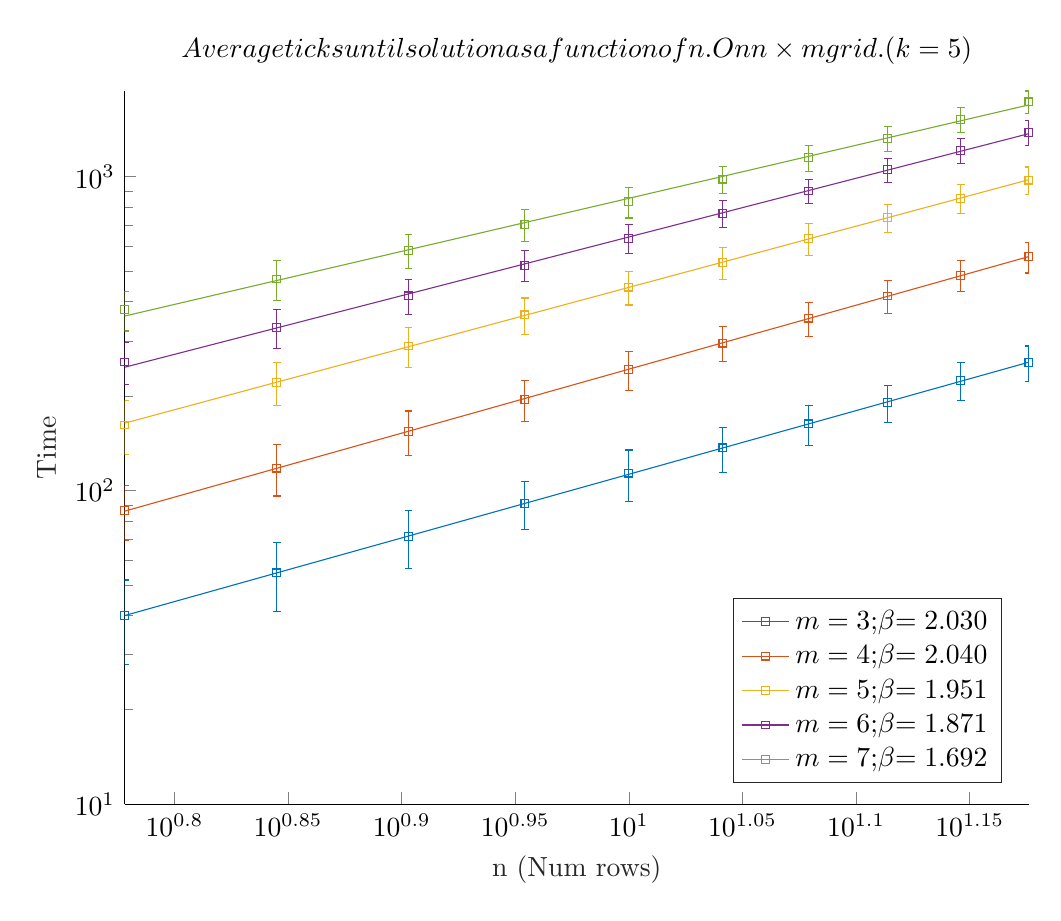
\begin{tikzpicture}

\begin{axis}[%
width=4.521in,
height=3.566in,
at={(0.758in,0.481in)},
scale only axis,
xmode=log,
xmin=6,
xmax=15,
xminorticks=true,
xlabel style={font=\color{white!15!black}},
xlabel={n (Num rows)},
ymode=log,
ymin=10,
ymax=1877.62135124314,
yminorticks=true,
ylabel style={font=\color{white!15!black}},
ylabel={Time},
axis background/.style={fill=white},
title style={font=\bfseries},
title={$\text{Average ticks until solution as a function of n. On n }\times\text{ m grid. (k = 5)}$},
axis x line*=bottom,
axis y line*=left,
legend style={at={(0.97,0.03)}, anchor=south east, legend cell align=left, align=left, draw=white!15!black}
]
\addplot [color=mycolor1, draw=none, mark size=1.4pt, mark=square, mark options={solid, mycolor1}]
 plot [error bars/.cd, y dir = both, y explicit]
 table[row sep=crcr, y error plus index=2, y error minus index=3]{%
6	39.87	11.9709526527687	11.9709526527687\\
7	54.6	13.5817866961501	13.5817866961501\\
8	71.374	15.1548494854239	15.1548494854239\\
9	90.742	15.8550370671532	15.8550370671532\\
10	113.546	21.0706389949453	21.0706389949453\\
11	136.656	22.3573111694016	22.3573111694016\\
12	163.044	23.9380057699149	23.9380057699149\\
13	190.74	25.8749962485354	25.8749962485354\\
14	224.654	31.0558079981964	31.0558079981964\\
15	255.43	33.2311558546927	33.2311558546927\\
};
\addlegendentry{$\text{m = 3; }\beta\text{ = 2.030}$}

\addplot [color=mycolor1, forget plot]
  table[row sep=crcr]{%
6	39.9282839422319\\
7	54.5950915295782\\
8	71.5899574093511\\
9	90.9221179362177\\
10	112.599745226953\\
11	136.630170358052\\
12	163.020042635421\\
13	191.775447301704\\
14	222.901995029718\\
15	256.404891578238\\
};
\addplot [color=mycolor2, draw=none, mark size=1.4pt, mark=square, mark options={solid, mycolor2}]
 plot [error bars/.cd, y dir = both, y explicit]
 table[row sep=crcr, y error plus index=2, y error minus index=3]{%
6	86.474	17.0141201526596	17.0141201526596\\
7	117.85	21.8657660155526	21.8657660155526\\
8	154.456	24.8082034399074	24.8082034399074\\
9	195.29	29.1407664370221	29.1407664370221\\
10	242.642	34.0002038777337	34.0002038777337\\
11	294.888	37.3626469991295	37.3626469991295\\
12	354.16	44.1140623951366	44.1140623951366\\
13	416.606	50.5974205066212	50.5974205066212\\
14	485.398	55.0017634623467	55.0017634623467\\
15	555.786	62.5315327589078	62.5315327589078\\
};
\addlegendentry{$\text{m = 4; }\beta\text{ = 2.040}$}

\addplot [color=mycolor2, forget plot]
  table[row sep=crcr]{%
6	85.9026214977235\\
7	117.642286067471\\
8	154.473697506816\\
9	196.424056238479\\
10	243.517459740575\\
11	295.775550289356\\
12	353.217977722003\\
13	415.862741799322\\
14	483.726452753791\\
15	556.824534259433\\
};
\addplot [color=mycolor3, draw=none, mark size=1.4pt, mark=square, mark options={solid, mycolor3}]
 plot [error bars/.cd, y dir = both, y explicit]
 table[row sep=crcr, y error plus index=2, y error minus index=3]{%
6	161.644	31.3810580702949	31.3810580702949\\
7	221.38	34.6054138732464	34.6054138732464\\
8	288.6	41.8843718014537	41.8843718014537\\
9	362.958	47.8984002812098	47.8984002812098\\
10	444.712	54.4520256942238	54.4520256942238\\
11	533.07	63.0339881915675	63.0339881915675\\
12	636.62	74.2982642066977	74.2982642066977\\
13	741.686	75.4632414199869	75.4632414199869\\
14	854.076	92.1685646661878	92.1685646661878\\
15	975.69	98.5692126343652	98.5692126343652\\
};
\addlegendentry{$\text{m = 5; }\beta\text{ = 1.951}$}

\addplot [color=mycolor3, forget plot]
  table[row sep=crcr]{%
6	163.893759723499\\
7	221.386819965668\\
8	287.258836569291\\
9	361.454595677932\\
10	443.925731312767\\
11	534.629237921352\\
12	633.526418591147\\
13	740.582114035778\\
14	855.764120688621\\
15	979.042740818152\\
};
\addplot [color=mycolor4, draw=none, mark size=1.4pt, mark=square, mark options={solid, mycolor4}]
 plot [error bars/.cd, y dir = both, y explicit]
 table[row sep=crcr, y error plus index=2, y error minus index=3]{%
6	256.79	39.659900597844	39.659900597844\\
7	330.746	47.5775654428317	47.5775654428317\\
8	417.06	53.2196303831231	53.2196303831231\\
9	522.352	58.2592514263057	58.2592514263057\\
10	635.976	67.6280898819578	67.6280898819578\\
11	762.868	74.6740316173969	74.6740316173969\\
12	900.878	81.4358318273401	81.4358318273401\\
13	1052.474	91.8290284437871	91.8290284437871\\
14	1214.118	110.87082915499	110.87082915499\\
15	1383.794	128.621999679694	128.621999679694\\
};
\addlegendentry{$\text{m = 6; }\beta\text{ = 1.871}$}

\addplot [color=mycolor4, forget plot]
  table[row sep=crcr]{%
6	247.086610588949\\
7	329.704615804065\\
8	423.295717217188\\
9	527.672281551231\\
10	642.671592030399\\
11	768.150250186518\\
12	903.980253492732\\
13	1050.04614352893\\
14	1206.24286950178\\
15	1372.47414761377\\
};
\addplot [color=mycolor5, draw=none, mark size=1.4pt, mark=square, mark options={solid, mycolor5}]
 plot [error bars/.cd, y dir = both, y explicit]
 table[row sep=crcr, y error plus index=2, y error minus index=3]{%
6	377.246	54.7472374098275	54.7472374098275\\
7	472.358	68.2851342175603	68.2851342175603\\
8	581.354	71.8934072639211	71.8934072639211\\
9	704.34	82.6729098316981	82.6729098316981\\
10	833.164	93.9654197256013	93.9654197256013\\
11	982.628	96.8527879881739	96.8527879881739\\
12	1150.17	110.722771661157	110.722771661157\\
13	1323.426	122.506588608552	122.506588608552\\
14	1523.172	134.655749069674	134.655749069674\\
15	1732.586	145.035351243138	145.035351243138\\
};
\addlegendentry{$\text{m = 7; }\beta\text{ = 1.692}$}

\addplot [color=mycolor5, forget plot]
  table[row sep=crcr]{%
6	359.753937617176\\
7	466.927836941604\\
8	585.256657746795\\
9	714.288558061358\\
10	853.640532528112\\
11	1002.98179942017\\
12	1162.02240044032\\
13	1330.50506451006\\
14	1508.1992139101\\
15	1694.89643149113\\
};
\end{axis}
\end{tikzpicture}%